\section{Evidence for the affine decision analysis}
\label{sec:flat-evidence}

\subsection{Controlled geometry and fixed-horizon sensitivity}

The reflection criterion predicts preservation for the equal-mass
corners of a rectangle at every bandwidth. A common equilibrium alone
does not imply preservation. For example, the six equal-mass sites
$\{\pm(1,0),\pm(0,1),\pm(3/5,4/5)\}$ have a common circumcenter at
the origin, which is the unique attracting equilibrium when
$\beta\ge1$. On the face $x=s(2,1)$ for $s>0$, the two competing
sites are $(1,0)$ and $(3/5,4/5)$. With normal $(-1,2)/\sqrt5$,
these sites and their antipodes cancel in the numerator of
\eqref{eq:facetvelocity}. The remaining two terms are proportional
to $(2/\sqrt5)(e^{s/\beta}-e^{-s/\beta})>0$. This gives crossing
even though the long-time limit is on the boundary of every cell.

To check \eqref{eq:sensitivity}, we fixed a nearest-corner classifier
with sites $(\pm1,\pm0.75)$ and $\beta=2$. We multiplied only the
upper-right site's driving weight by $e^\varepsilon$. We measured
switches in $[-0.30,0.30]\times[0.30,1.20]$ under a standard
bivariate Gaussian feature law. These are unconditional masses
within that rectangle. On the central vertical facet the base normal
derivative is $-0.5$ and its tangential dynamics is one-dimensional.
We integrated the response along that base path. A separate full
two-dimensional solve and a bracketed root at each quadrature node
located the initial abscissas whose terminal abscissa was zero.
The endpoint remains in the upper half-plane on this strip.
This isolates the one boundary relevant to the label comparison.

At horizons $0.25$, $0.75$, and $1.50$, the predicted coefficients
of $|\varepsilon|$ in the strip switch mass were $0.00875$,
$0.02897$, and $0.06830$. Across both perturbation signs and the three
horizons the relative errors were $1.54$--$2.03\%$ at
$|\varepsilon|=0.08$. They decreased at every tested magnitude,
reaching $0.098$--$0.124\%$ at $|\varepsilon|=0.005$.
Doubling the quadrature order and tightening the solver tolerances
for the smallest perturbation at the longest horizon changed
the mass coefficient by less than $2\times10^{-14}$. The symmetric
control's numerical switch mass was below $2\times10^{-17}$.
This calibration uses an unlabeled feature law and one fixed geometry.

\begin{figure}[htbp]
\centering
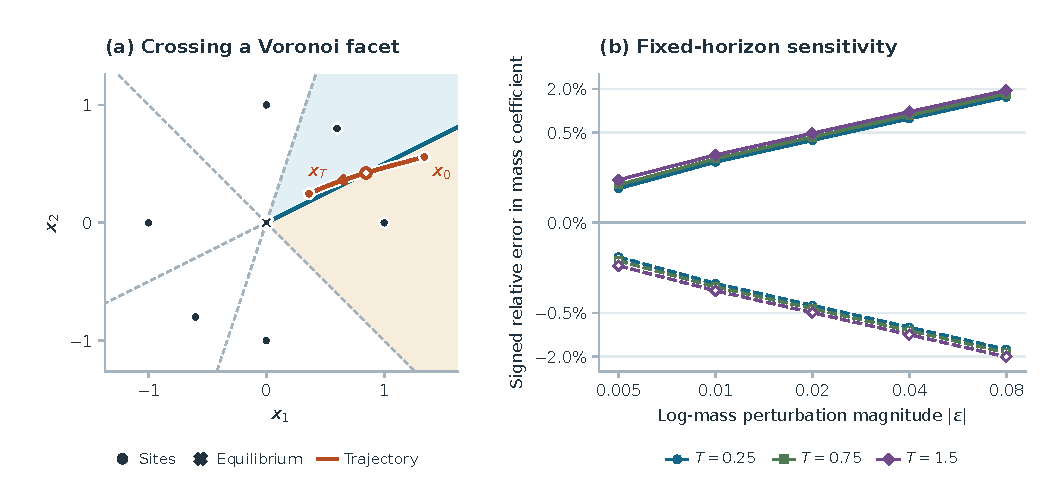
\includegraphics[width=\linewidth]{figures/decision_invariance.pdf}
\caption{Examples of preservation and its failure. The cospherical
configuration in panel (a) has a shared stationary point and a permeable
Voronoi facet. The trajectory starts at $(3,1.25)/\sqrt 5$ with
$\beta=1.2$ and crosses at $t\approx0.7483$ over $[0,2.25]$.
Panel (b) checks the limiting switch-mass coefficient
under a fixed readout and a perturbation of the driving mixture at
three fixed positive horizons.}
\label{fig:decision-invariance}
\end{figure}

\subsection{Outward-rounded reachability on two fixtures}
\label{sec:interval-check}

We compared the preservation inequalities with a small verified
integrator on exact decimal inputs. The cases use the cospherical
six-site example and the reflection-symmetric rectangle. The
17 fixed queries include points close to active boundaries and
are observed at $T=0.50,1.25,2.25$. The benchmark fixes the step
$h=1/64$ and uses 38-digit decimal interval arithmetic. Basic
operations round outwards, and the exponential is rounded to
nearest and widened to the two neighboring representable numbers.

Given an initial box $X$, the prototype hull and variation of
constants supply a bounding box $Y$ for the entire step. Two
intersections with $X+[0,h]F(Y)$ tighten it. The endpoint enclosure
then uses
\[
 e^{-h}X + (1-e^{-h})\mu(X)
   + (h-1+e^{-h})D\mu(Y)F(Y),
\]
intersected with $Y$. The last term encloses the drift remainder
by integrating the derivative of $\mu$ along the flow with the
positive exponential kernel. We check all affine margins over
these boxes. Preservation requires a strict decision throughout
all step tubes. A certified different label at any stored
endpoint proves departure by the observation horizon.
This is a fixed-step interval enclosure, with wrapping and
dependency limitations familiar from validated ODE integration
\cite{neher}.

All 51 query--horizon endpoints received a strict interval label,
with 10 changes and 41 original labels. Interval tubes certified
whole-horizon preservation on 29 rows and departure on 10.
They left the whole-path result unresolved on 12 rows with certified
endpoint labels. These unresolved rows record the limits of the tube
enclosures.
The original whole-plane implementation, which includes nonfacet
rival bisectors, confirmed preservation for two rows. A separate
check using only the actual Voronoi facets confirmed all 27
rectangle rows and none of the 24 cospherical rows. On the
cospherical fixture, the established floating-point local and
covariance tests accepted one and two rows, respectively.
The interval integrator certified ten departures on that fixture.
These are deliberately difficult exact-input cases. They establish
valid enclosures for the reported fixtures. Section~\ref{sec:verified-public}
reports separate outward-rounded certificates on the public cohorts.

\subsection{External one-prototype cohorts}

We added a descriptive check on Iris, Letter Recognition and
UCI Human Activity Recognition (HAR) \cite{iris,letter,har},
with one equal-mass centroid per class fitted after training-only
standardization. Iris used three disjoint stratified test folds
after exact-feature deduplication. Letter Recognition retained the
original 16,000-row training set and the source test set, with 380
test rows removed because their exact feature vectors occurred in
training. The remaining 3,620 rows were partitioned into disjoint
test folds. Font grouping is unavailable and some quantized feature
vectors may repeat within test. HAR used the original 21 training
subjects and nine held-out subjects, with the latter divided into
three disjoint blocks and up to 16 windows per subject and activity.
Its 864 windows may overlap in time and are not independent subjects.
The design compares three horizons ($0.15$, $0.50$, $1.25$) and two
bandwidths ($\sqrt{\beta}/D=0.35$, $0.60$). The comparisons pool
test rows within each source and quantify performance on these
cohorts.

For each strict initial winner, the plane conditions use all rival
bisectors and cancel the two equal-mass sites defining each plane.
The global test keeps other sites as separate terms, which yields a
conservative envelope even when more projections coincide. The local
test bounds relative logits on the projected trajectory tube by
\eqref{eq:local-plane}. We compare both with the covariance-based
whole-interval test of Section~\ref{sec:bounds}, the union of all
three conditions, and ETD1 as an endpoint
approximation. Numerical departures are sampled at 12 checkpoints
per horizon increment. A refined RK4 integration independently checks
the DOP853 endpoints. Table~\ref{tab:flat-transfer} shows an
intermediate horizon.

\begin{table}[htbp]
\centering\small
\setlength{\tabcolsep}{4pt}
\begin{tabular}{lrrrrrrr}
\toprule
Source & Switch & $\Delta$ accuracy & ETD1 & \multicolumn{4}{c}{Preservation coverage (\%)}\\
\cmidrule(lr){5-8}
 & (\%) & (pp) & agreement (\%) & Global & Local & Cov. & Union\\
\midrule
Iris (149) & 2.68 & $+1.34$ & 100.00 & 49.66 & 96.64 & 93.29 & 97.32\\
Letter (3,620) & 19.75 & $-1.38$ & 98.26 & 8.73 & 65.06 & 14.75 & 65.06\\
HAR (864) & 6.37 & $-1.74$ & 99.77 & 32.29 & 86.23 & 30.32 & 86.23\\
\bottomrule
\end{tabular}
\caption{Endpoint disagreement with the initial label, change in ordinary
accuracy, ETD1 agreement with the numerical endpoint, and analytical
whole-interval preservation tests at $\sqrt{\beta}/D=0.35$ and $T=0.50$.
Parenthetical counts are held-out evaluation rows or windows.
Accuracy changes are in percentage points.}
\label{tab:flat-transfer}
\end{table}

There were no sampled certificate contradictions or solver endpoint
disagreements across the 18 source--bandwidth--horizon combinations.
At the intermediate horizon and smaller bandwidth, the local
plane test covered 50.31 and 55.91 percentage points more queries
than the covariance test on Letter and HAR. At the longest horizon,
the global plane and covariance tests returned no certificates on
these sources. The local test still covered 13.37\% of Letter and
44.79\% of HAR queries at the larger bandwidth.
At that bandwidth and horizon, 72.90\% of Letter and 33.22\% of HAR queries switched
labels, and accuracy fell by 33.81 and 26.04 percentage points.
The global plane test's conservative offsets in this evaluation are
bandwidth independent after canceling the tied pair. It cannot
adapt to changes in the relative driving weights of the remaining
prototypes. In addition, splitting an exact projection group
can loosen the whole-plane bound under an arbitrarily small
prototype perturbation. These checks evaluate prediction behavior
and certificate coverage. The exact-arithmetic guarantees are
separate from the floating-point evaluations.

\paragraph{Computational cost.}
On the first held-out fold of each source, we timed the optimized
local plane test followed by RK4 only on remaining queries, and
compared with RK4 on the full fold. The timing used one thread,
batches of at most 64, warm-up, and 15 interleaved repeats.
At $\sqrt{\beta}/D=0.35$ and $T=0.50$, the median hybrid to full-RK4
latency ratios were 1.04 on Iris, 2.03 on Letter, and 0.34 on HAR.
The methods agreed on all endpoint labels in these folds.
The timing excludes a one-time setup (0.04, 3.64, and 0.15 ms,
respectively) and compares against RK4 with maximum step 0.10.
These machine- and batch-specific results show that stronger
coverage can accompany either a gain or a loss in latency.

To isolate class count, a synthetic diagnostic used dimensions
16 and 128 and $K\in\{3,6,12,26,40\}$ equal-mass sites. Standardized
Gaussian site draws and nearly balanced class assignments were
shared between two query regimes with coordinate noise standard
deviations $0.08D$ and $0.45D$. Each setting used 256 queries per
seed over three seeds. Among the 15,360 query appearances,
no sampled departure contradicted the local certificate and the
hybrid agreed with full RK4 throughout. For $K=3$, hybrid to
full-RK4 ratios ranged from 0.145 to 0.697 across regimes and
dimensions. For $K=40$, they ranged from 1.33 to 2.46, with local
coverage between 77\% and 100\%. This implementation processes
$O(K^2)$ rival--site terms per query after scoring and uses a
one-time $O(K^4)$ projected-logit calculation for setup.
The experiment characterizes these costs on fixed synthetic cases.
